\section{Software Architecture Document}
\label{sec:Software Architecture Document}
% 
% \subsection{Architektonische Repr\"asentation}
% 
% 
% \subsection{Architektonische Faktoren}
% 
% 
\subsection{Architektonische Entscheidungen}
% 
\subsubsection{Matrixmultiplikation}
Brainstorming zu Beginn des Projektes: Kybernetisches System mit
\begin{itemize}
  \item Operand: Graph als Adjazenz-Matrix
  \item Operator: e.g. Dijkstra-Algorithmus (als Matrix)
  \item Transition: Ein Schritt der Traversierung
  \item Transformierte: Graph im neuen Zustand
\end{itemize}
Berechnung der Traversierung per Matrixmultiplikation:
\begin{itemize}
  \item Definition der Operatoren (Algorithmen) allgemein g\"ultig als Matrizen
  \item Anwenden der Operatoren (Algorithmen) auf Operanden (Graphen) als Matrixmultiplikation
  \item Resultat: Liste von (bijektiven, also eineindeutigen) Transformationen ('Steps') als Matrizenmechanik
\end{itemize}
% 
\subsubsection{Entscheidungen}
% 
\begin{itemize}
  \item Themenkreis Matrizen: Entscheid, dass keine Matrizen-Multiplikation. Implementation mit Bezug auf \textit{Algorithm Design} von M. Goodrich und R. Tamassia~\cite{goodrichtamassia:2002}.
  \item Zu Projektbeginn wurde relativ bald eine Drei-Schichten-Architektur entworfen.
  \item In der Woche 45 wurde entschieden, das Projekt als Maven-Projekt zu halten. Der Entscheid wurde vorallem getroffen, da Properties zentral verwaltet und Tests sauber vom restlichen Sourcecode getrennt gehalten werden k\"onnen.
\end{itemize}
% 
% \subsection{Logical View}
% 
% \subsubsection{Beschreibung und Motivation}
% 
% \subsection{Deployment View}
% 
% \subsubsection{Beschreibung und Motivation}
% 
\subsection{Process View}
% 
\begin{figure}[H]
    \centering
    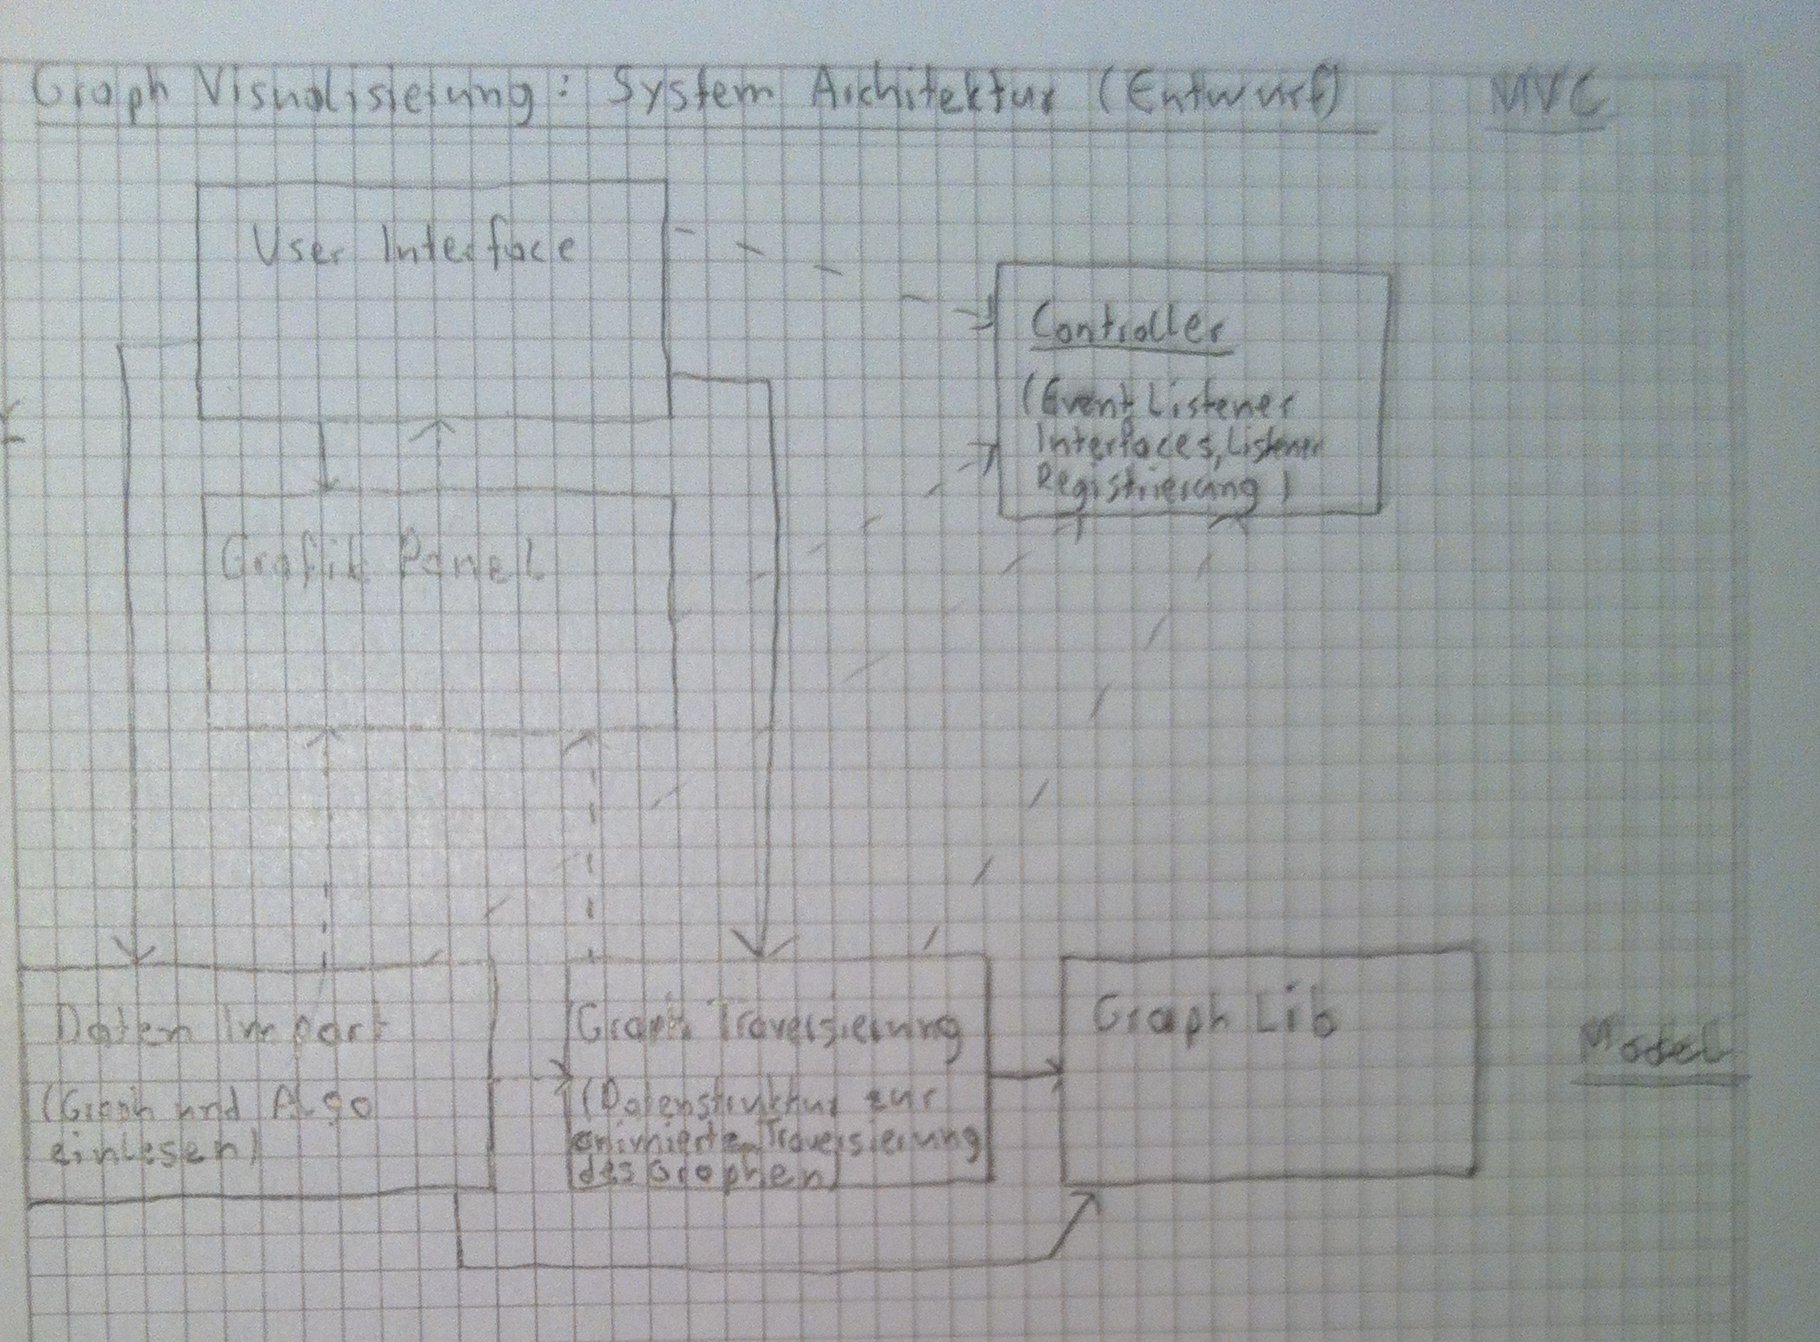
\includegraphics[
% 		    width=\textwidth,
% 		    height=\textheight,
% 		    angle=90,
		    scale=0.1,
		    keepaspectratio=true
    ]{diagrams/Draft_System_Architecture_PK_V1_cropped.jpeg}
    \caption{Gui, MVC: Conceptual Class Diagram}
    \label{fig:gui-mvc-ccd}
\end{figure}
% 
\subsection{Use-Case View}
Folgende Use Cases wurden implementiert:
\begin{itemize}
  \item Daten:
  \begin{itemize}
    \item Neuen Graphen oder Algorithmus importieren
    \item Importierter Graph oder Algorithmus l\"oschen
  \end{itemize}
  \item Traversierung:
  \begin{itemize}
    \item Graph ausw\"ahlen
    \item Algorithmus ausw\"ahlen
%     \item evt. Start- resp. Endknoten ausw\"ahlen
  \end{itemize}
  \item Visualisierung:
  \begin{itemize}
      \item Einstellen Steplength: Anzahl Traversierungs-Schritte pro Bild
      \item Einstellen Delay: Zeitintervall zwischen zwei Bildern (in Sekunden)      
      \item Visualisierung, Step-by-Step: Ein Bild vor, ein Bild zur\"uck, an das Ende oder den an den Anfang springen
      \item Visualisierung, Animation: Starten, Anhalten, Stoppen
  \end{itemize}
\end{itemize}
% 
\begin{figure}[H]
    \centering
    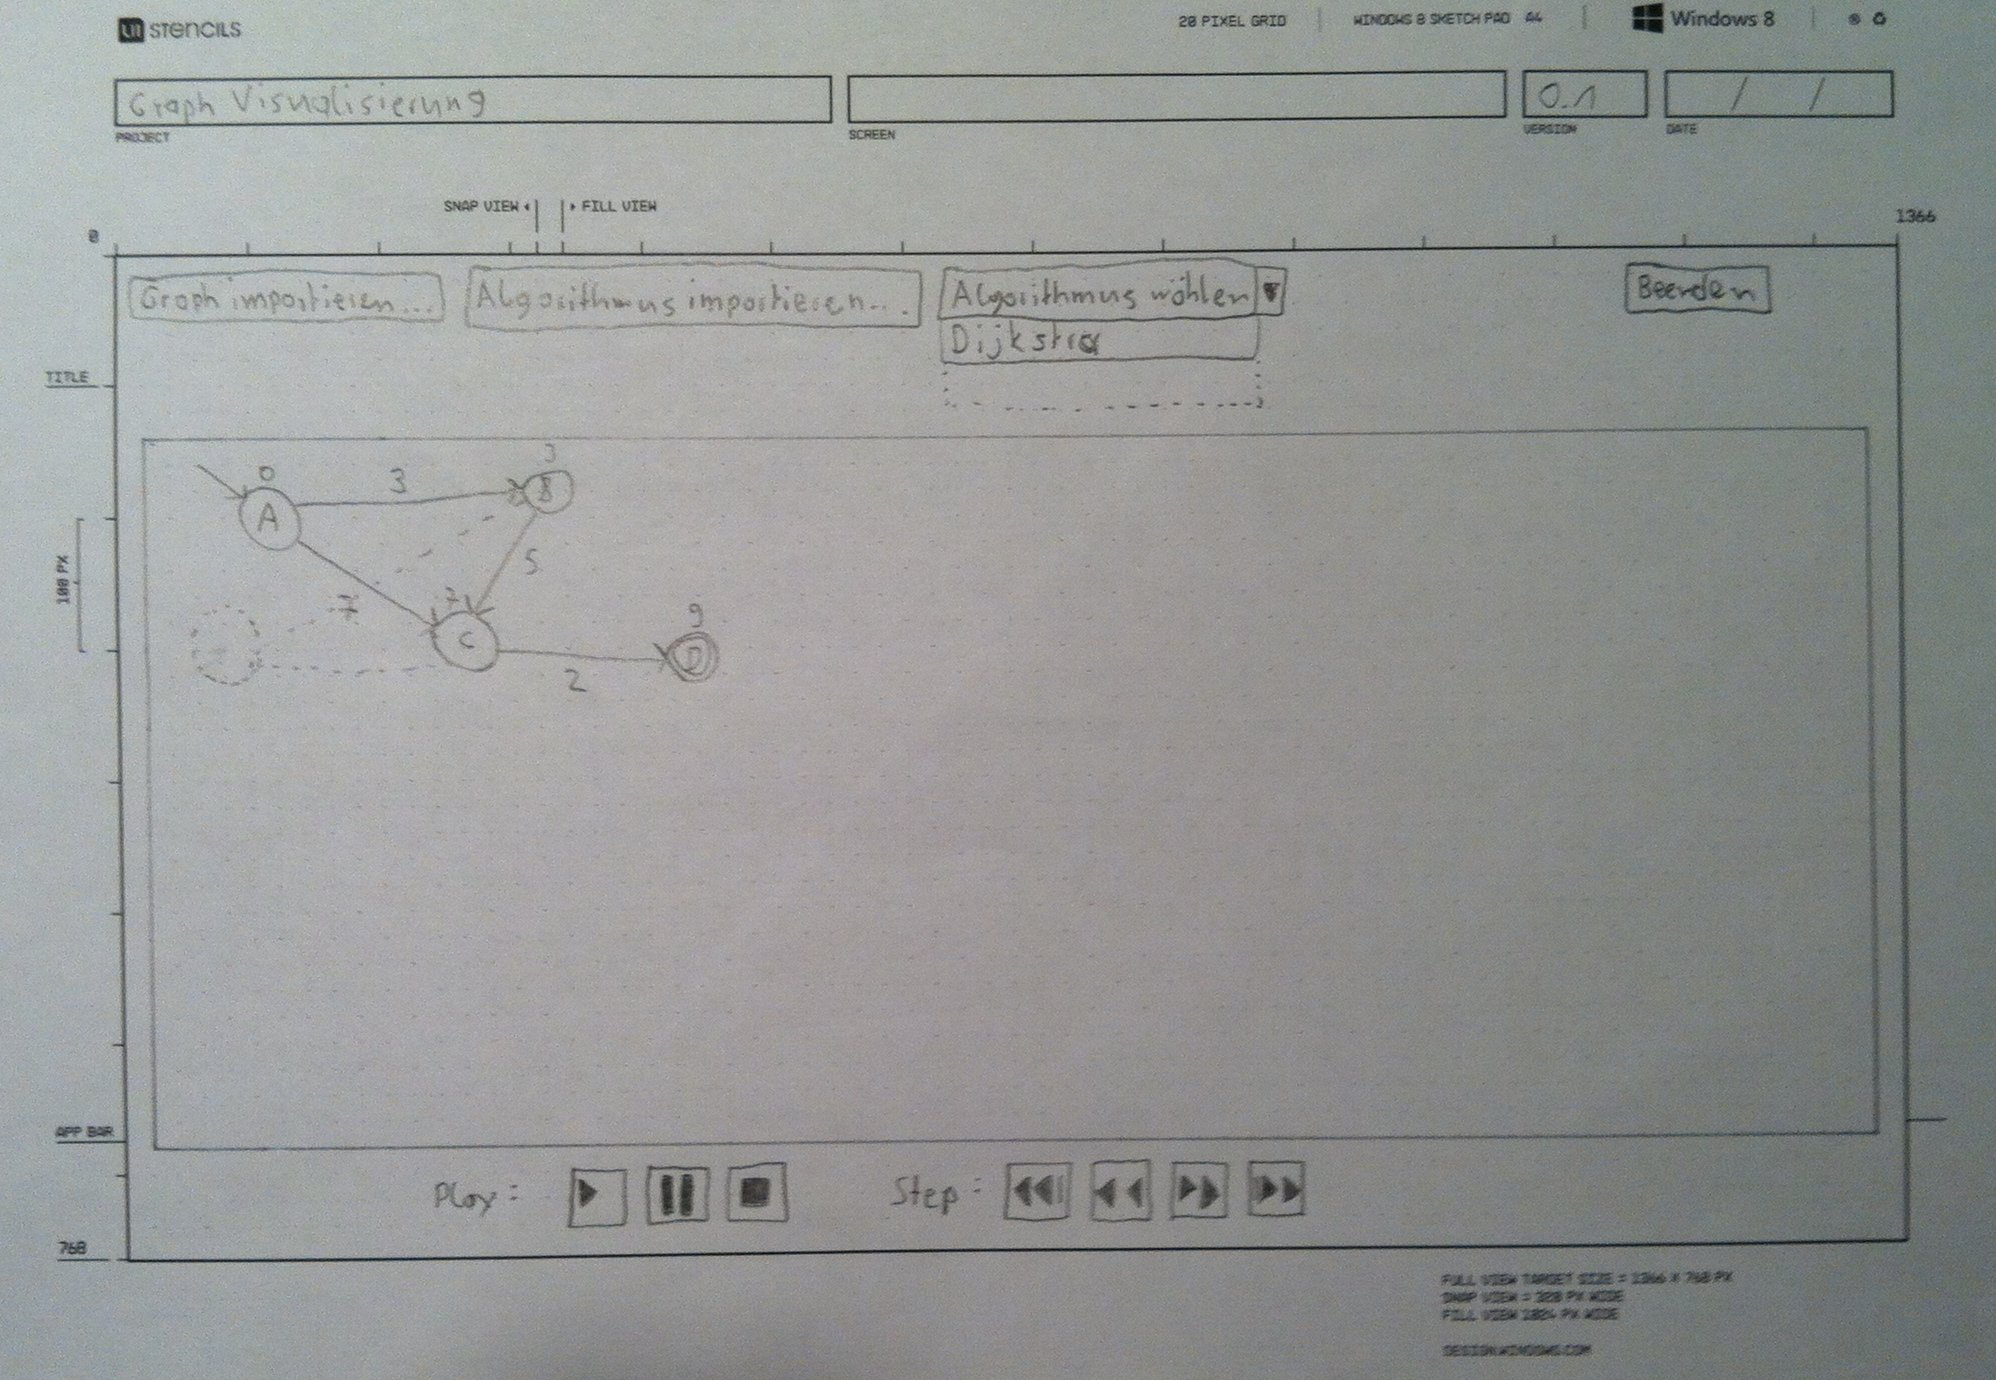
\includegraphics[
% 		    width=\textwidth,
% 		    height=\textheight,
% 		    angle=90,
		    scale=0.1,
		    keepaspectratio=true
    ]{diagrams/Screen_Sketch_PK_V1_cropped.jpeg}
    \caption{Gui, View: Screen Sketch}
    \label{fig:gui-view-screen-sketch}
\end{figure}
% 
\begin{figure}[H]
    \centering
    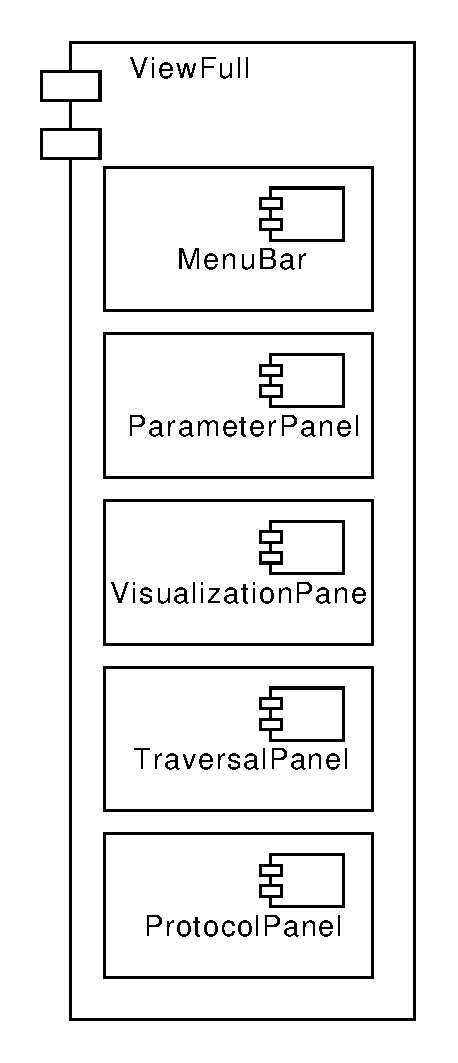
\includegraphics[scale=0.5]{diagrams/designmodel/cd-view-full.pdf}
    \caption{Gui, View: Component Diagram}
    \label{fig:gui-view-cd}
\end{figure}